\chapter{Construção das Ferramentas de Apoio}
\label{sec:ferramentas}

Este capítulo aborda o ferramental e \textit{wiki} criados para dar apoio às melhorias propostas no Método FreeTest 2.0. As ferramentas criadas neste trabalho estão sob licença \textit{Creative Commons} e oferecidas de maneira \textit{aaS} (\textit{As-a-Service}), deste modo, poderão ser acessadas na web de forma gratuita e sob demanda, não sendo necessário sua instalação ou configuração em ambiente local. Todo o código fonte gerado neste trabalho é distribuído de maneira \textit{open-source}. 

O capítulo é organizado da seguinte maneira, nas seções \ref{sec:arquiteturaplataforma} e \ref{sec:implementacaoplataforma} assuntos relevantes a arquitetura e de implementação da ferramenta são abordados. Enquanto que o capítulo \ref{sec:aspectosoperacionais} mostra de forma prática as funcionalidades e aspectos operacionais da ferramenta criada, utilizando elementos de UML para facilitação do entendimento e layouts de tela da ferramenta. Por fim, as considerações finais deste capítulo são expostas na seção \ref{sec:consideracoesfinaiscap6}.

\section{Arquitetura da Plataforma Web}
\label{sec:arquiteturaplataforma}

A arquitetura da plataforma web é baseada no modelo MVC (\textit{Model View Controller}) \cite{Reenskaug1979} (vide figura \ref{fig:fig61}) de padrão de projetos. Este \textit{design pattern} \footnote{https://pt.wikipedia.org/wiki/Padr\%C3\%A3o_de_projeto_de_software} separa a lógica de negócios da interface do usuário, ideal para aplicações que serão evoluídas e na organização do projeto, além de ser um padrão amplamente utilizado pela indústria. Na \textbf{camada de apresentação} (\textit{view}) todo o layout foi desenvolvido com base nas boas práticas de UX (\textit{User Experience}) \footnote{https://pt.wikipedia.org/wiki/Experi\%C3\%AAncia_do_usu\%C3\%A1rio} e UI (\textit{User Interface}) \footnote{https://pt.wikipedia.org/wiki/Interface_do_utilizador} utilizando um padrão de \textit{front-end} \footnote{https://pt.wikipedia.org/wiki/Front_end} amplamente conhecido na comunidade mundial chamado Bootstrap \footnote{https://github.com/twbs/bootstrap/blob/master/LICENSE} que é distribuído sob a licença MIT \footnote{https://pt.wikipedia.org/wiki/Licen\%C3\%A7a_MIT}, que diferente de licenças \textit{copy right} podem ser distribuídos em software livres ou proprietário sem nenhum ônus. Abaixo desta camada está a \textbf{camada de negócios} (\textit{controller}) que representa as principais funcionalidades do software, desde o cadastro de usuários que terão acesso aos dados da empresa, manutenção dos dados da empresa, criação/manutenção das áreas de processo e práticas especificas, área de modelagem dos processos, o guia de implantação e por fim a \textit{dashboard} principal, que mostra o o resultado da implantação do processo na Organização. A camada \textit{controller} também controla todas as requisições realizadas pelo usuário através da camada anterior. Por fim, a \textbf{camada de modelo} (\textit{model}) que é responsável por gerenciar toda a leitura e escrita dos dados e também suas validações.

\begin{figure}[H]
\centering
\includegraphics[width=.90\textwidth]{fig/figura61.png}
\caption{Esquema da arquitetura em três camadas da ferramenta.}
\label{fig:fig61}
\end{figure}


Todo o ferramental foi projetado com base nos padrões da UML (\textit{Unified Modeling Language}) \footnote{http://www.uml.org/} e funciona de forma \textit{As-A-Service} (Como um serviço). A ferramenta foi distribuída "como um serviço" com o intuito de reduzir custos para as MPEs, desta forma, toda a plataforma opera \textit{on cloud}, bastando somente um rápido cadastro para que a Organização possa utilizar os recursos da ferramenta, caso prefira mantê-la em seu ambiente operacional basta baixar o código fonte e utilizá-lo em sua infraestrutura local. Na figura \ref{fig:fig62} é apresentado o diagrama de caso de uso geral do sistema, onde o usuário inicialmente faz um registro da sua empresa e cadastro pessoal do seu usuário para uso da ferramenta (i), neste registro inicial o usuário em questão terá perfil de administrador na plataforma. Após o login (ii) é possível atualizar os dados da empresa (iii) e cadastrar novos usuários (iv), neste caso o usuário em questão serão os colaboradores da Organização que terão acesso a ferramenta. Como mencionado anteriormente a plataforma permite que os usuários modelem os processos da Organização (v), desta forma é possível manter centralizado todos os processos (não somente o processo de teste) em um só lugar. Como funcionalidades principais a plataforma web possui ainda o guia de implantação (vi), manutenção do guia de implantação (vii) e \textit{dashboard} de status geral de implantação (viii) que serão melhor explicados nas seções seguintes.

\begin{figure}[H]
\centering
\includegraphics[width=.90\textwidth]{fig/figura62.png}
\caption{Diagrama de Caso de Uso: Principais funcionalidades da ferramenta.}
\label{fig:fig62}
\end{figure}

\section{Aspectos Relevantes de Implementação}
\label{sec:implementacaoplataforma}

Conforme supracitado na seção \ref{sec:arquiteturaplataforma}, a ferramenta foi desenvolvida com base nos padrões de projeto MVC, por se tratar de um padrão amplamente utilizado pela indústria e por guiar na criação de uma arquitetura facilmente escalável e organizada. Como linguagem de desenvolvimento foi escolhido o Node.js \footnote{http://nodejs.org/}, que é uma linguagem amplamente utilizada na indústria para desenvolvimento de sistemas web e escaláveis, basicamente a linguagem consiste em um interpretador Java Script Engine que trabalha no lado do servidor. Para armazenamento dos dados foi utilizado o MongoDB \footnote{http://www.mongodb.org/}, por ser uma aplicação de código fonte aberto, alta performance e bem escalável e amplamente utilizada no contexto web. Abaixo segue alguns dos principais \textit{frameworks} que foram utilizados e seus propósitos:

\begin{itemize}
    \item Bootstrap \footnote{http://getbootstrap.com/} - Utilizado como layout padrão;
    \item BPMN.io \footnote{https://bpmn.io/toolkit/bpmn-js/} - Utilizado na criação da funcionalidade de modelagem dos processos;
\end{itemize}

\section{Aspectos Operacionais}
\label{sec:aspectosoperacionais}

Essa seção é destinada a apresentação das principais funcionalidades da plataforma web. A plataforma é dividida em dois módulos (vide figura \ref{fig:fig63}), um \textbf{Módulo de Processo}, que consiste de uma área para manutenção do processo que é disponibilizado em uma \textit{wiki} e a funcionalidade de modelagem que pode ser acessada dentro da plataforma web e que serão melhor explicados na seção \ref{sec:ferramentaprocesso}. O \textbf{Módulo FreeTest Wizard} que abrange as funcionalidades do \textit{wizard} de implantação, com um guia para implantação passo-a-passo e área para manutenção da Áreas de Processo e Práticas Especificas, sendo que o mesmo será explicado na seção \ref{sec:oguiadeimplantacao}.

Todo o arcabouço é entregue de forma gratuita, sob a licença \textit{Creative Commons}\footnote{https://creativecommons.org/} e disponibilizado na web como uma proposta \textit{As-a-Service} (como serviço). 

%A ferramenta é dividida em três partes:

%\begin{itemize}
    % \item \textbf{Módulo de Processo} - As funcionalidades de processo, compreendem as telas onde a Organização poderá modelar seus processos e/ou instanciar o processo de teste modelo já entregue.
    % \item \textbf{Módulo de Implantação} - O guia de implantação é a principal função do software. Tem como objetivo auxiliar as Organizações na implantação do FreeTest de forma mais didática possível. O guia de implantação é totalmente customizável para crescer conforme as necessidades da empresa, caso o processo mude ou evolua o guia de implantação pode ser alimentado com as novas informações;
    % \item \textbf{Módulo para manutenção dos dados da organização} - Funcionalidade que mantem a tela de cadastro da organização, seus integrantes e cadastro/recuperação de dados de acesso.
%\end{itemize}

\begin{figure}[H]
\centering
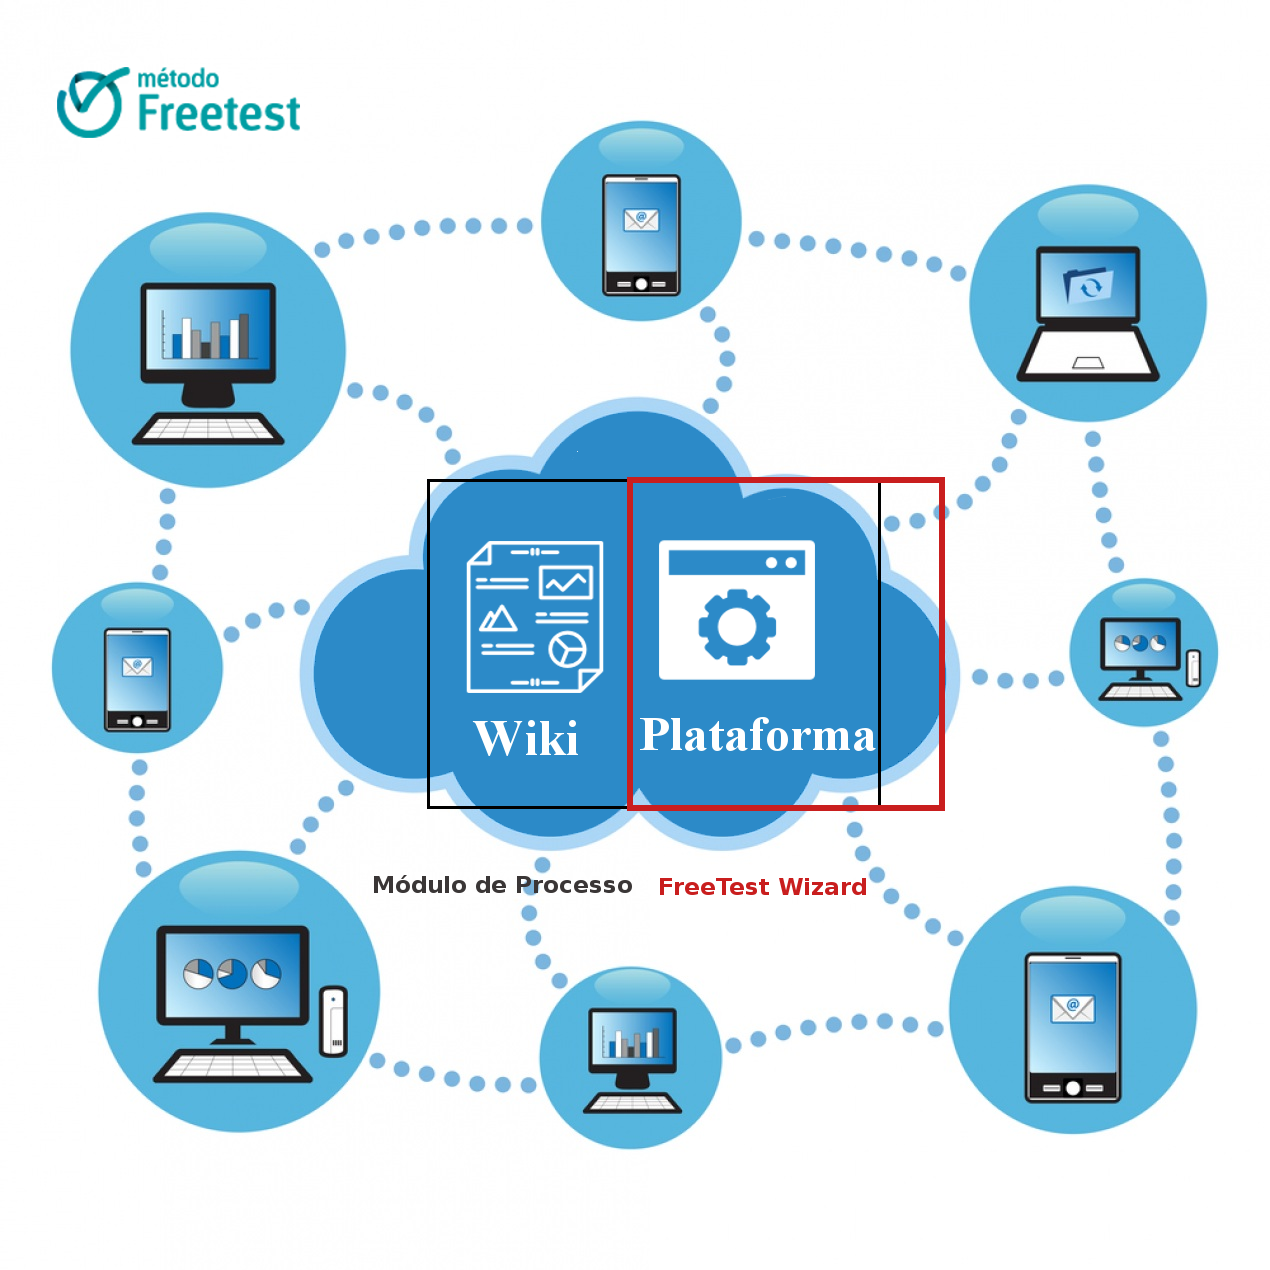
\includegraphics[width=.75\textwidth]{fig/figura63.png}
\caption{Módulos do Sistema: Módulo de Processo e Módulo FreeTest Wizard.}
\label{fig:fig63}
\end{figure}

\subsection{Módulo de Processo}
\label{sec:ferramentaprocesso}

O Módulo do Processo é dividido em duas partes, sendo a primeira uma \textit{wiki}\footnote{http://wiki.freetestframework.com} que contempla toda a parte informativa do processo (vide seção \ref{sec:wikiprocesso}) e a segunda, o Gestor de Processos (vide seção \ref{sec:gestordeprocessos}), uma área do software \footnote{http://freetestframework.com} que abrange toda a manutenção das áreas de processo, práticas especificas e uma funcionalidade para modelagem de todos os processos da Organização. 

\subsubsection{Construção da \textit{Wiki} para o Processo}
\label{sec:wikiprocesso}

Uma ferramenta tipo \textit{wiki} foi escolhida pois é mais fácil para manter o processo de teste organizado e para se usar esse tipo de ferramenta como gestora de conhecimento. A velocidade em que processos das MPEs precisam se adaptar aos novos cenários do mercado é bem grande. Uma solução eficiente é a \textit{wiki}, que pode prover informações para novos colaboradores e manter os processos atualizados e acessíveis. 

Alguns benefícios de se utilizar uma \textit{wiki} como ferramenta para manutenção do processo podem ser vistos a seguir:

\begin{itemize}
	\item Os processos de teste ficam armazenados numa central de conhecimento;
    \item Novos colaboradores tem um local fácil para aprendizado;
    \item Mudanças são facilmente inseridas;
    \item Aumentamos a eficiência no tempo de aprendizado dos colaboradores;
    \item Ferramenta amplamente conhecida, facilitando a absorção de conhecimento.
\end{itemize}

A \textit{wiki} do processo matem todo o processo FreeTest 2.0, tela de boas vindas, parte informativa do guia de implantação e lista de ferramentas sugeridas para auxilio da execução de cada prática especifica do processo. Se tratando do processo, a estrutura é organizada em Áreas de Processos (AP) e suas respectivas Práticas Especificas (PE) (conforme apresentado na seção \ref{sec:areasdeprocessoepraticas}). No interior de cada PE contém a sua descrição detalhada, dependências, resultados gerados para aquela prática e por fim uma seção que é destinada à parte didática e prática de como implantar (visto na seção \ref{sec:estruturaguiaimplantacao}) a determinada Prática Especifica. A estrutura para cada Prática Especifica (PE) pode ser vista na figura \ref{fig:fig64}.

\begin{figure}[H]
\centering
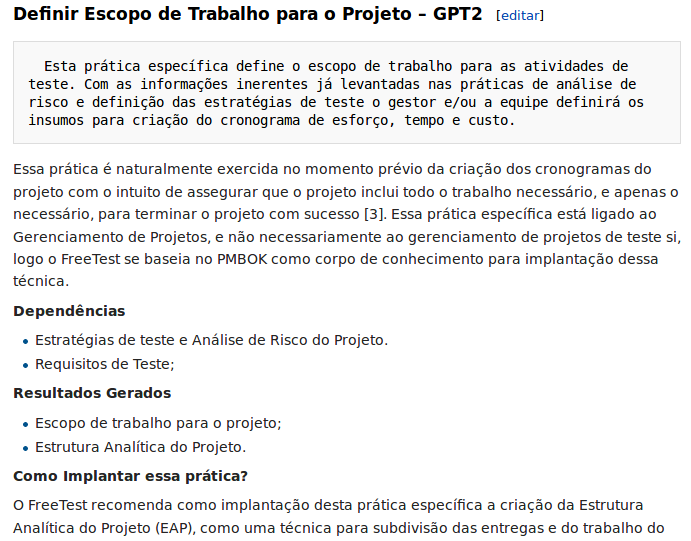
\includegraphics[width=.90\textwidth]{fig/figura64.png}
\caption{Estrutura de uma Prática Especifica do processo.}
\label{fig:fig64}
\end{figure}

Para a criação da wiki do processo do Método FreeTest 2.0 foram utilizados o software Wikimedia \footnote{https://commons.wikimedia.org}, que é distribuído sob licença \textit{Creative Commons} e \textit{open-source} e banco de dados MySQL Server \footnote{https://dev.mysql.com/downloads/mysql/}.

\subsubsection{Construção do Gestor do Processos} 
\label{sec:gestordeprocessos}

Como mencionado o gestor de processos integra uma das partes do módulo de processo. Com a finalidade de criar um ambiente onde as Organizações pudessem manter todos os seus processos, e não somente o processo de teste a ferramenta permite que sejam criados quantas modelagens de processo forem necessários. A modelagem dos processos é feita em BPMN \footnote{http://www.bpmn.org/} (\textit{Business Process Model and Notation}) utilizando o \textit{framework} BPMN.io que foi incorporado à plataforma e que já mencionado na seção \ref{sec:aspectosoperacionais}. A seguir na figura \ref{fig:fig65} é mostrado a interface da ferramenta de modelagem.

\begin{figure}[H]
\centering
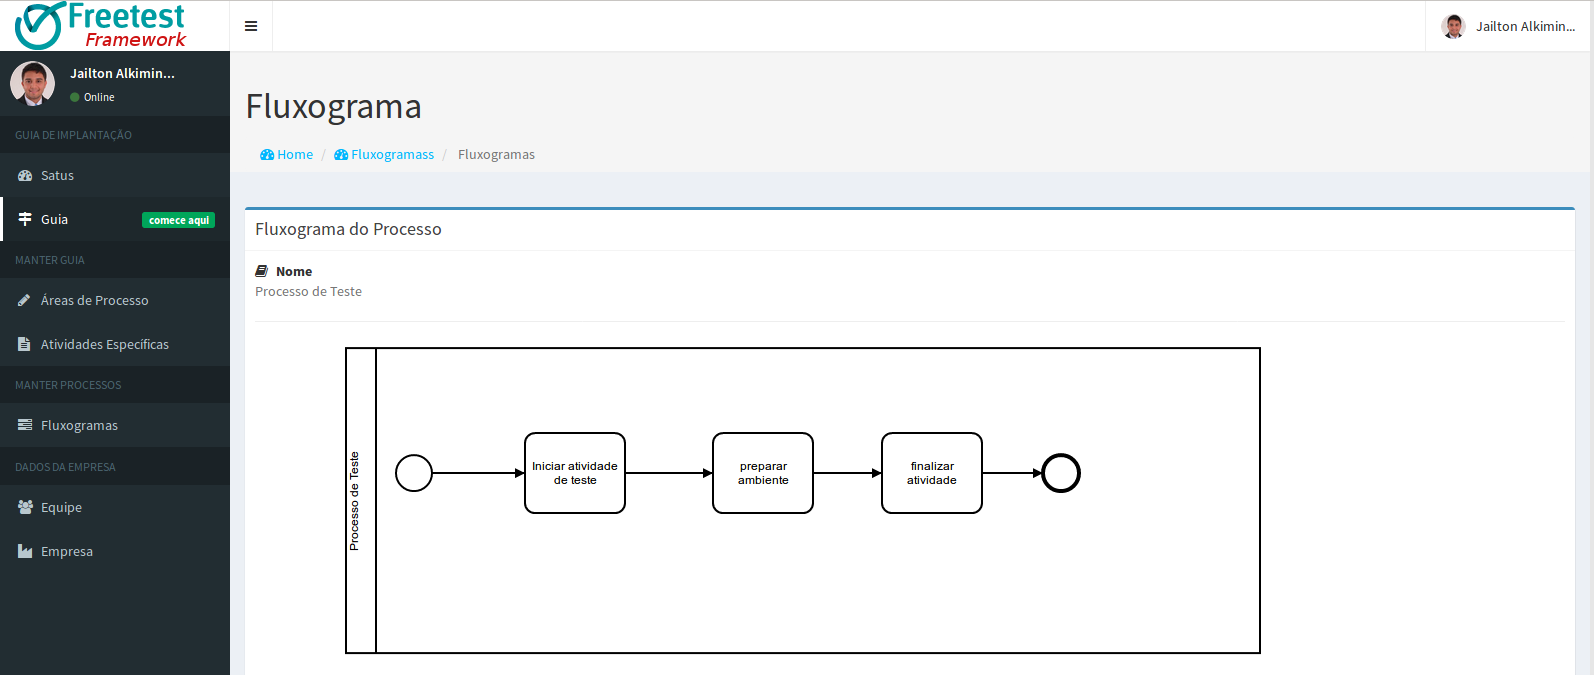
\includegraphics[width=.90\textwidth]{fig/figura65.png}
\caption{Área para modelagem dos processo.}
\label{fig:fig65}
\end{figure}

Como um dos entregáveis deste trabalho foi feita uma modelagem de processo de teste padrão. A modelagem deste processo padrão foi elaborada dentro do contexto do novo processo (seção \ref{sec:areasdeprocessoepraticas}) e entregue como um "modelo de processo de teste" para as Organizações que desejam começar com o nível de maturidade inicial, podendo evoluí-lo conforme suas necessidades. Desta maneira toda Organização recém cadastrada poderá decidir em usar o processo de teste padrão ou criar o seu a partir do zero. A modelagem do processo básico entregue como padrão na ferramenta pode ser vista na figura \ref{fig:fig66}.

\begin{figure}[H]
\centering
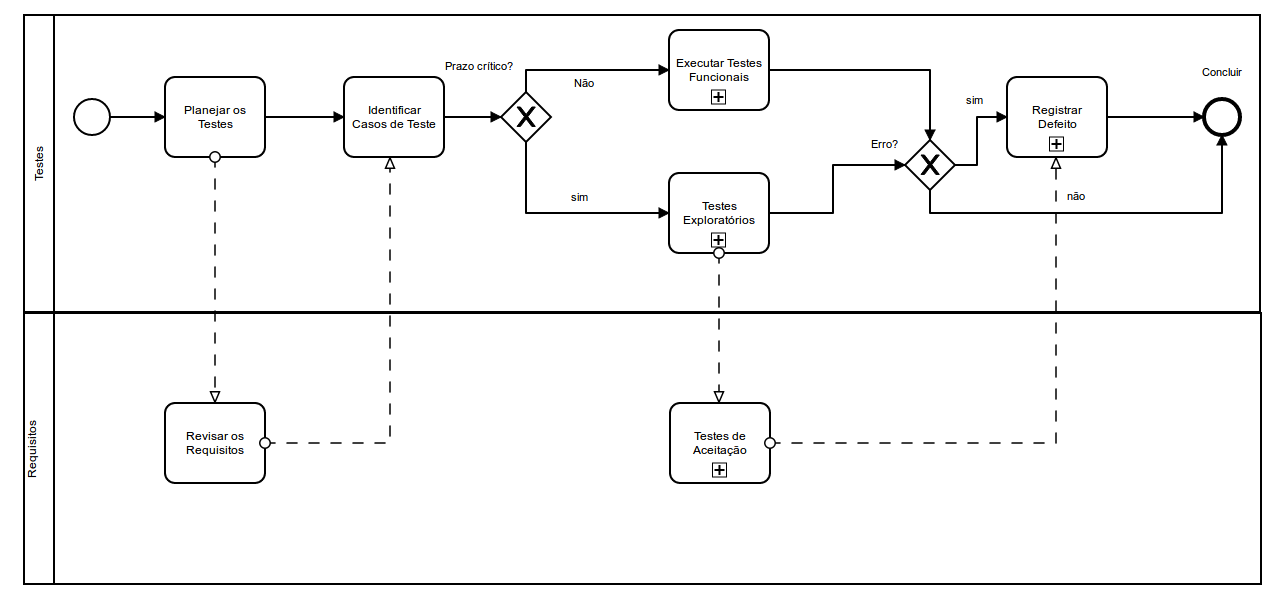
\includegraphics[width=.90\textwidth]{fig/figura66.png}
\caption{Modelagem do processo de teste básico entregue junto com a ferramenta.}
\label{fig:fig66}
\end{figure}

\subsection{Módulo FreeTest Wizard}
\label{sec:oguiadeimplantacao}

Como apoio à proposta principal deste trabalho, foi criado um módulo do sistema \footnote{http://guide.freetestframework.com} que servirá como o guia de implantação do processo. O \textbf{FreeTest Wizard}, como foi nomeado, é entregue na mesma plataforma web e no formato \textit{As-a-Service} de forma gratuita. Essa ferramenta representa um grande diferencial desta pesquisa, pois através dela será possível que mesmo MPEs com poucos recursos na área de qualidade de software, possam facilmente implantar, monitorar e definir os marcos para a implantação de seus processos de teste, além de contar com o apoio do guia. O funcionamento geral do FreeTest Wizard pode ser visto no caso de uso da figura \ref{fig:fig67}. Para maior facilidade na implantação do processo FreeTest 2.0 o FreeTest Wizard vem com com informações das Áreas de Processo e Práticas Especificas já populadas, desta maneira auxiliando as Organizações que não possuem nenhum nível de maturidade em teste à implantar o FreeTest 2.0 até um nível básico inicial.

\begin{figure}[H]
\centering
\includegraphics[width=.90\textwidth]{fig/figura67.png}
\caption{Modelagem do Caso de Uso representativo do Guia de Implantação.}
\label{fig:fig67}
\end{figure}

O FreeTest Wizard também é dividido em duas partes. Uma parte refere-se ao \textit{"status"} da implantação do processo na Organização e a outra corresponde aos passos necessários para se alcançar um objetivo na implantação de uma prática especifica. Como será visto adiante.

\subsubsection{\textit{Status} Geral de Implantação}
\label{sec:statusimplantacao}

O \textit{status} geral da implantação do processo tem como finalidade exibir indicadores do percentual de que cada área de processo foi implantada. Os indicadores de cada Área de Processo contabilizam quantas práticas especificas foram implantadas e exibem um gráfico tipo "barra" com o percentual de implantação respectivo.

O progresso de cada Área de Processo tem como finalidade dar uma visão geral para a equipe da Organização de como está a implantação do processo. Desta maneira, aumenta o engajamento da equipe e facilita na obtenção de indicadores para metas e planejamento. A figura \ref{fig:fig68} exibe a tela que contempla o \textit{status} geral de implantação.

\begin{figure}[H]
\centering
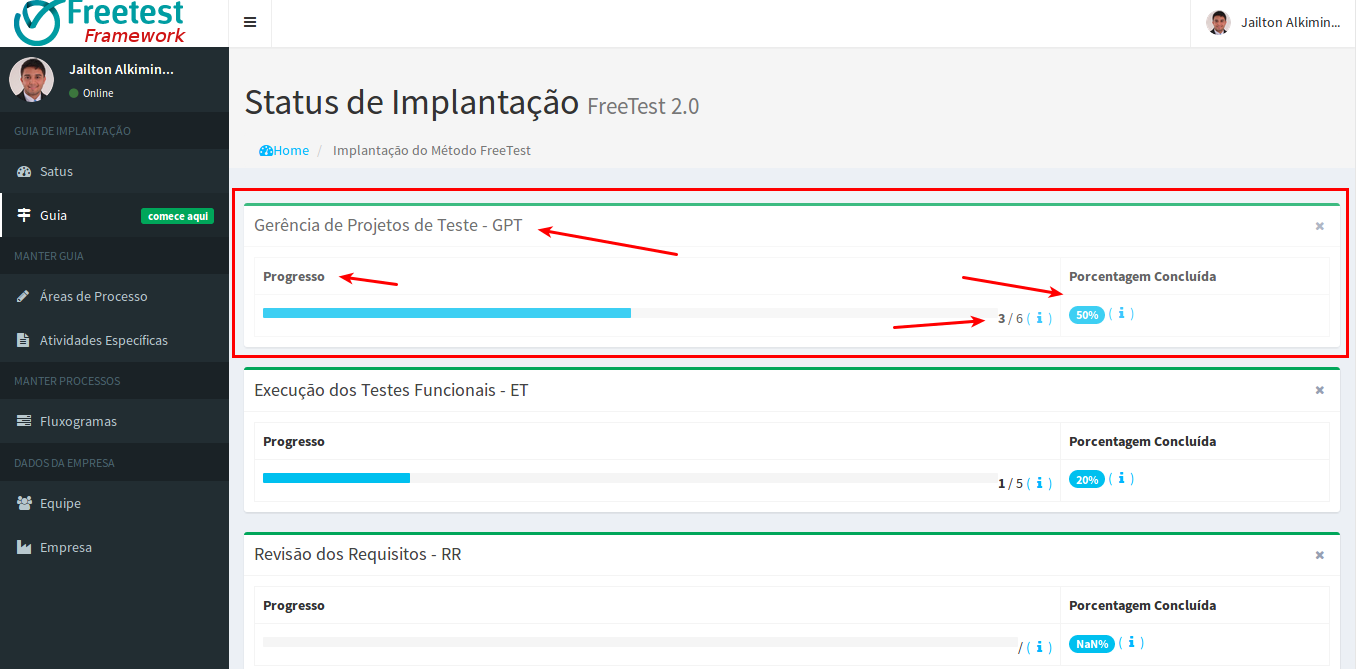
\includegraphics[width=.90\textwidth]{fig/figura68.png}
\caption{Status geral da implantação do processo.}
\label{fig:fig68}
\end{figure}

\subsubsection{Guia de implantação}
\label{sec:passoapassoguia}

O passo a passo do guia de implantação auxiliará a Organização a realizar as tarefas/sugestões disponibilizadas na seção \ref{sec:estruturaguiaimplantacao} para alcançar o nível de maturidade desejado, área de processo que deseja implantar e/ou somente determinada Prática Especifica. O guia de implantação é totalmente customizável, o que permite que as Organizações possam futuramente estender o processo do Método FreeTest 2.0 e ajustá-lo, desta forma inserindo novas áreas de processo e práticas especificas adequadas às necessidades da Organização.

Como mencionado, é possível atualizar e customizar o guia de implantação. Neste sentido duas funcionalidades do guia de implantação foram criadas para a manutenção e customização das áreas de processo e suas respectivas práticas especificas, através delas é possível facilmente realizar ajustes necessários e adequações ao processo da Organização. As Figuras \ref{fig:fig69} e \ref{fig:fig610} mostram respectivamente as telas para criação de áreas de processos e suas práticas especificas.

\begin{figure}[H]
\centering
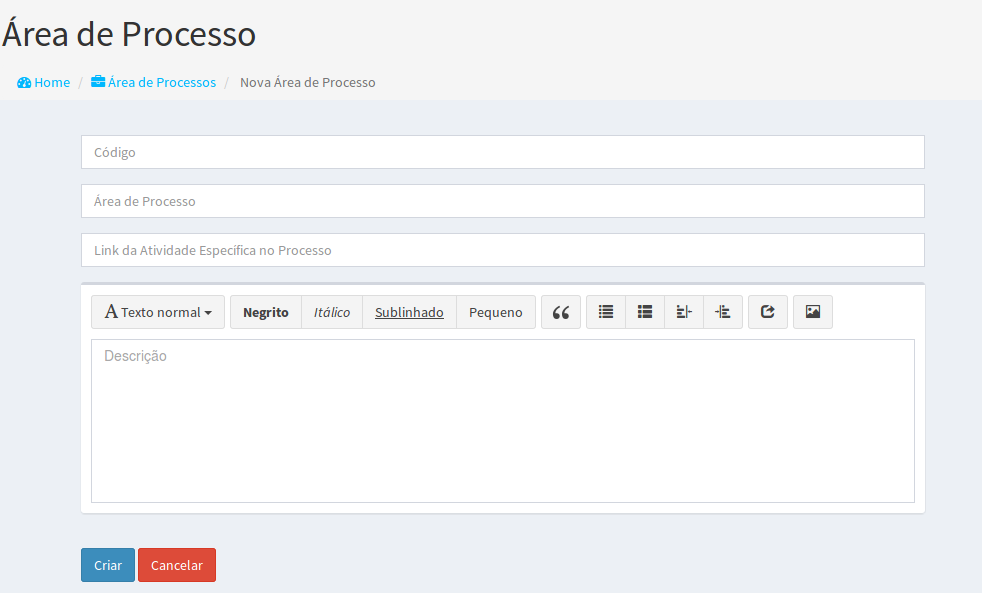
\includegraphics[width=.90\textwidth]{fig/figura69.png}
\caption{Funcionalidade para a criação/manutenção de uma Área de Processo.}
\label{fig:fig69}
\end{figure}

Perceba que na figura \ref{fig:fig69} que mostra a tela de criação de uma área de processo requer que o usuário da aplicação informe o código, titulo, link e descrição objetiva da Área de Processo. O link para a área de processo será o link da AP na \textit{wiki} do Freetest 2.0 (mostrado na subseção \ref{sec:wikiprocesso}).

\begin{figure}[H]
\centering
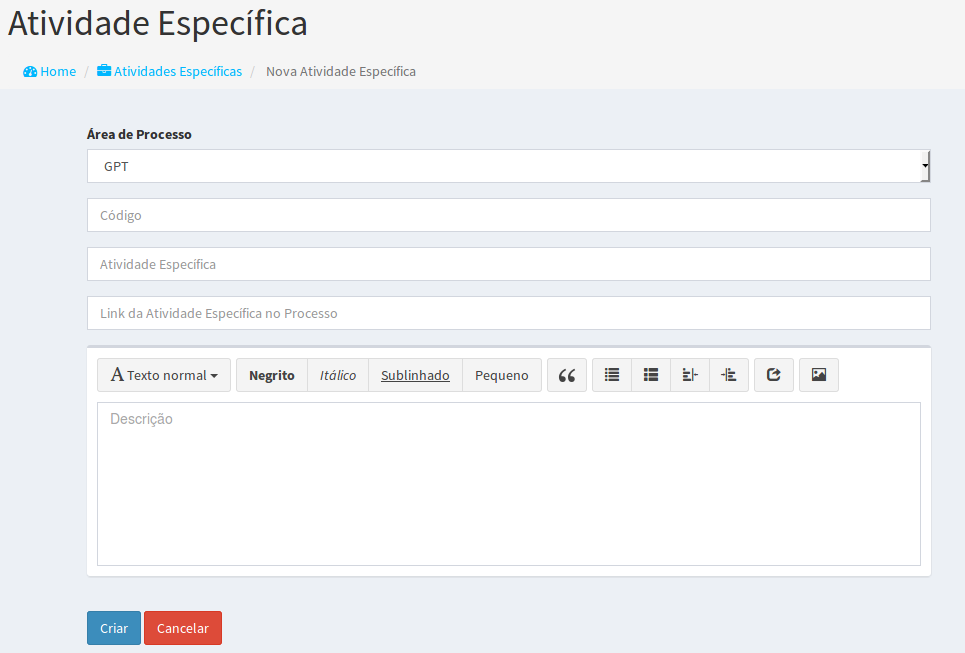
\includegraphics[width=.90\textwidth]{fig/figura610.png}
\caption{Tela para criação/manutenção das Práticas Especificas.}
\label{fig:fig610}
\end{figure}

Seguindo o mesmo padrão da tela de criação da área de processo visto na figura \ref{fig:fig69}, a tela para criação de uma prática especifica (figura \ref{fig:fig610}) requer que sejam informadas: área de processo no qual a prática especifica é vinculada, código da prática, título, link para a prática especifica (direcionado para a \textit{wiki}) e a descrição objetiva.

O passo a passo de implantação do FreeTest Wizard é apresentado na figura \ref{fig:fig611}. O passo a passo funciona como um guia para auxiliar os usuários na implantação das práticas especificas do processo do Método Freetest 2.0 ou até mesmo de práticas especificas criadas pela Organização. Assim que uma nova área de processo e suas práticas especificas são cadastradas, automaticamente elas são lançadas no Guia de Implantação, desta forma podendo ser executadas pela equipe responsável na implantação do processo, para então, os indicadores de implantação serem atualizados no \textit{Status} Geral de Implantação do Processo.

\begin{figure}[H]
\centering
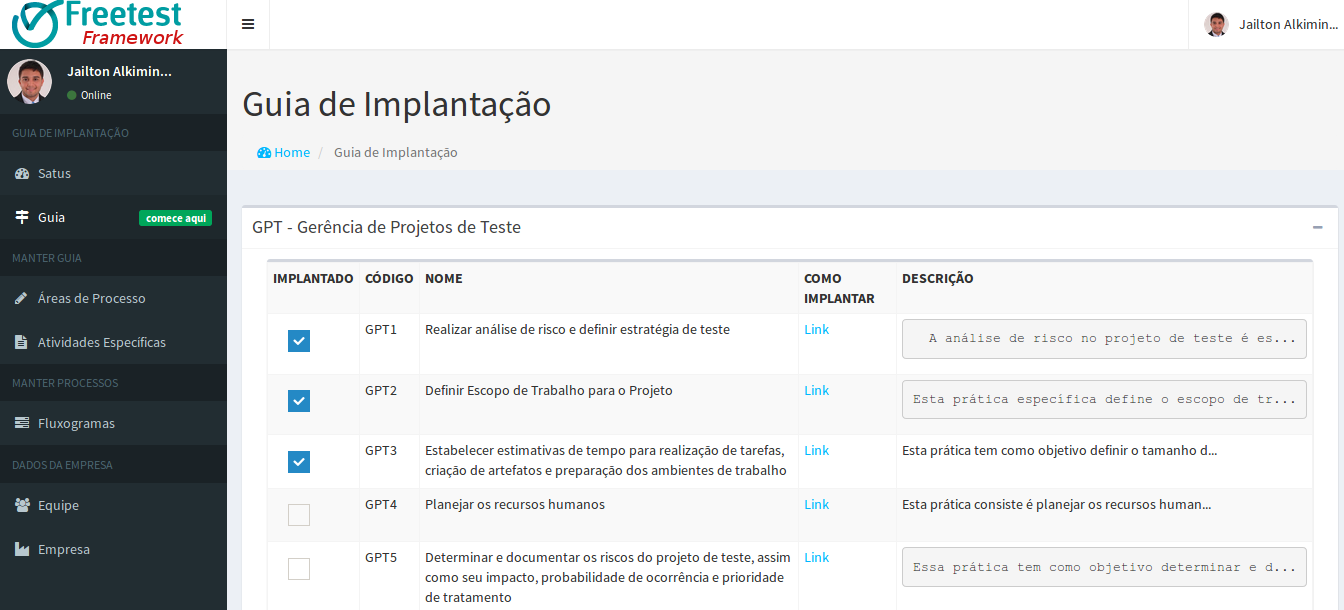
\includegraphics[width=.90\textwidth]{fig/figura611.png}
\caption{Guia de implantação.}
\label{fig:fig611}
\end{figure}


\section{Considerações Finais}
\label{sec:consideracoesfinaiscap6}

Com base no conhecimento empírico dos autores e de revisões da literatura do estado da prática de processos de teste em Organizações, principalmente MPEs observou-se que um dos grandes fatores de desistência na implantação de processos de teste é o custo de implantação e o \textit{know-how} técnico necessário para a implantação deste tipo de processo. A partir dessa premissa este trabalho, por meio deste capítulo propôs à criação de ferramentas que apoiassem as Organizações, não somente com um processo de teste, mas também com a sua implantação, manutenção e evolução do mesmo. 

Por fim, através da plataforma web que abrange o FreeTest Wizard e o Gestor de Processos em conjunto com a \textit{wiki} MPEs poderão de forma fácil, sob demanda e através da web gerenciar seus processos e implantar o processo FreeTest 2.0 intuitivamente. 
